\section{Types of faults}

In order to be able to analyze fault-tolerance techniques, we first need to understand the various types of faults that we might encounter. This list is not exhaustive and only covers fault types relevant to this thesis, for more complete list see \cite{1335465}. It is also important to understand two different classifications are not always mutually exclusive.

Faults can be further split into various categories, the ones mostly relevant to us are \textbf{external faults} which originate from outside the system boundaries and propagate into the system. Which also includes \textbf{natural faults} that are caused by natural phenomena without human participation. These faults can affect the hardware and the software, which is why we can further classify them as \textbf{hardware faults} and \textbf{software faults} respectively \cite{1335465}. \\

\subsection{Transient fault} 
Transient fault is a temporary fault which results in an error, such as a bit-flip in the register file \cite{shubu}. The most common subtype of transient fault is \acrfull{seu}, when talking about faults, we are referring to \acrshortpl{seu}, unless specified otherwise. A key characteristic of transient fault is the possibility to correct it by overwriting the corrupted region. Retrying the same process multiple times is usually enough to deal with a transient fault, since it is extremely unlikely a transient fault will occur repeatedly within the same process at successive time intervals. If a fault persists across multiple attempts, it is possible we are dealing with a permanent fault. \\

\subsection{Permanent fault} 
Permanent fault is a lasting fault within the system that requires maintenance to remove \cite{shubu}. This could come in various forms, such as damaged hardware, corrupted memory or missing code. When dealing with a permanent fault, retrying the same process is usually not enough as the same error will keep reoccurring. This approach requires alternatives and fallbacks within the system, which is outlined in more detail in section \ref{multi}. \\

\subsection{Hardware faults}

Hardware faults \cite{1335465} are caused by external factors beyond our control as software developers. They are usually caused by environmental influences, such as cosmic radiation in space, electromagnetic fields, adverse weather conditions or heavy system usage.

One of the most common hardware faults is memory corruption, which can appear in many forms and result from a wide range of causes. For instance, radiation exposure in space can cause \acrshortpl{seu}, flipping individual bits in memory and altering data unpredictably. Similarly, physical damage to storage media, such as hard drives or SSDs, might corrupt specific regions of the file system, making certain data inaccessible or incorrect.

% Memory corruption is not always catastrophic. While it can result in complete system failure and unrecoverable states, it is just as likely to manifest as small, hard-to-detect errors. These subtle corruptions might not immediately disrupt the software's functioning but can lead to unpredictable behavior over time.

\begin{figure}[!hbt]
    \centering
    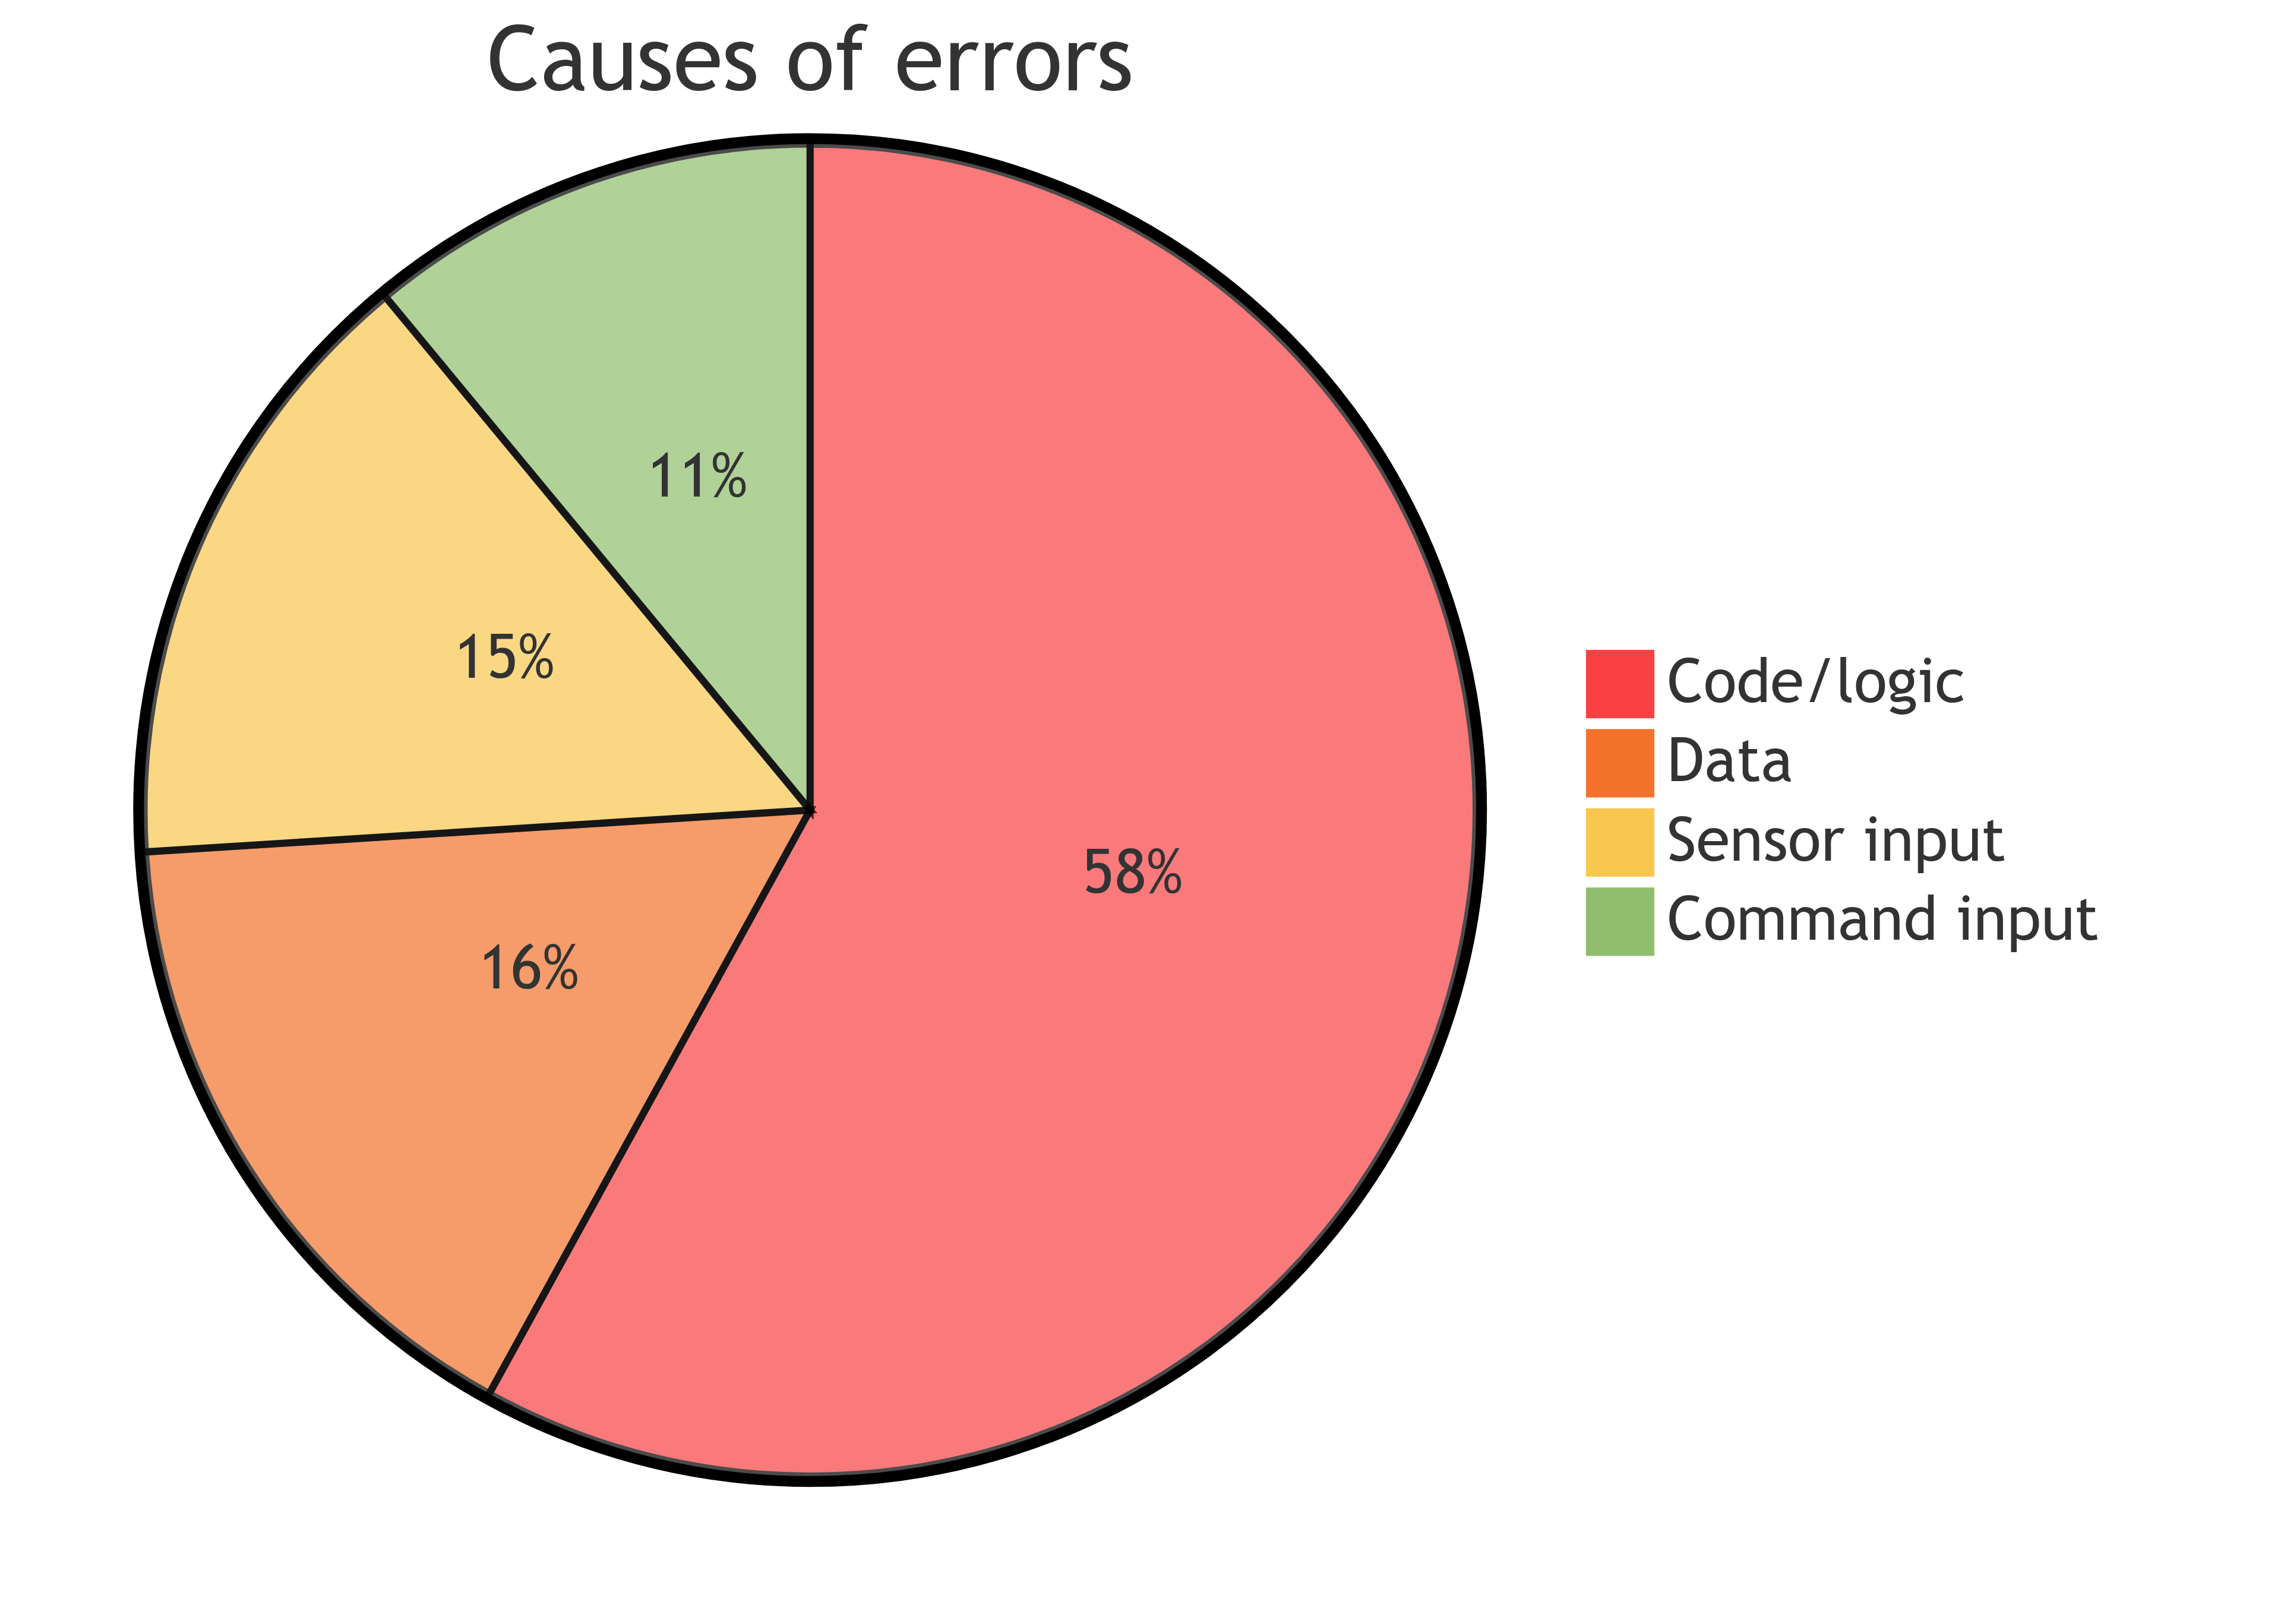
\includegraphics[width=0.6\textwidth]{diagrams/stats/piechart.png}
    \caption{Causes of errors \cite{nasa:stats}}
    \label{fig:nasa_stats}
\end{figure}

\subsection{Development faults}

Development faults is a category which includes all the various faults whose causes are introduced during software development stage \cite{1335465}. According to research conducted by NASA, majority of errors stem from faults within the code and logic of the afflicted software, followed closely by faults in data \cite{nasa:stats} (see Figure \ref{fig:nasa_stats}).
We are employing the use of a language with built-in static code analysis - Rust, to minimize the possibility of development faults, allowing us to focus on the main problem. 

% To ensure that software remains robust and as free of errors as possible, there are several effective strategies. One promising approach we will look at is the use of memory-safe programming languages, specifically Rust. Rust is a modern language that has gained traction for its safety features, particularly in system programming and embedded applications. It ensures high performance through zero-cost abstractions and introduces a memory ownership model, which reduces memory-related errors such as null pointer dereferencing and data races. This model makes Rust particularly well-suited for low-level and resource-constrained environments, where reliable memory management is crucial. (https://docs.rust-embedded.org/book/) \\